\documentclass[10pt]{gshs-report-v2.0}
% 추가로 필요한 패키지가 있다면 이곳에 적어 넣으시오.
\usepackage{enumitem}
\usepackage{multirow}
\usepackage{cite}
\usepackage{bm}
\usepackage{makecell}

\usepackage{amsmath, amsfonts, amsthm, amssymb}
\usepackage[utf8]{inputenc}
\usepackage[english]{babel}
\usepackage{hyperref}
\usepackage[capitalize,nameinlink]{cleveref}
\usepackage{graphicx, wrapfig}
\usepackage{caption, subcaption}
\usepackage{verbatim, listings, fancyvrb}

\theoremstyle{theorem}
\newtheorem{theorem}{Theorem}[section]
\theoremstyle{lemma}
\newtheorem{lemma}[theorem]{Lemma}
\theoremstyle{definition}
\newtheorem{definition}[theorem]{Defintion}

\newtheorem*{lambert}{램버트 코사인 법칙}

\hypersetup{
	colorlinks=true,
	linkcolor=black,
	citecolor=blue,
	urlcolor=cyan,
}

%%%%%%%%%%%%%%%%%%%%%%
%%%%%알앤이 정보%%%%%%
%%%%%%%%%%%%%%%%%%%%%%

%사업 시행 년도
\researchYear{2021}

%연구 종류: 기초 또는 심화
\researchtype{심화} 

%보고서 종류: 중간 또는 최종
\reporttype{중간} 


% 제목 및 영문 제목: 개행 시에는 \linebreak만 사용 가능하다.
\title{베지어 곡면을 이용한 3D 모델링} 
\englishtitle{Application of Bézier Curve to 3D Modeling}

% 제출 년월일
\summitdate{2021}{06}{21}

%연구 참여자 (저자 1, 2, 3)
\author[1]{박건호}
\email[1]{abc0004@naver.com}
\author[2]{윤상}
\email[2]{abc0004@naver.com}

%연구 책임자: 없는 경우 그대로 내버려 둘 것, 있는 경우 채울 것
\professor{}
\professorEmail{abc0004@naver.com}

%지도교사
\advisor{김소연}
\advisorEmail{abc0004@naver.com}




\graphicspath{{figures/}}
\renewcommand{\contentsname}{차례}
\renewcommand{\listfigurename}{그림 목차}
\renewcommand{\figurename}{그림}
\renewcommand{\tablename}{표}
\setlength{\tabcolsep}{10pt}
\renewcommand{\arraystretch}{1.5}


%%%%%%%%%%%%%%%%%%%%%%%%%%
%%%%%%%%문서 시작%%%%%%%%%
%%%%%%%%%%%%%%%%%%%%%%%%%%
\begin{document}


%%%%%%%%%%%%%%%%%%%%%%
%%%%%제목 페이지%%%%%%
%%%%%%%%%%%%%%%%%%%%%%
\makecover


%%%%%%%%%%%%%%%%%%%%%%%%%%%%%
%%%%%요약문(국문) 페이지%%%%%
%%%%%%%%%%%%%%%%%%%%%%%%%%%%%
\noindent{
\huge 베지어 곡면을 이용한 3D 모델링
}\\
\vspace{10pt}
\noindent{
\Large Application of Bézier Curve to 3D Modeling
}

\begin{abstractkor}
\noindent{
본 연구에서는 베지어 곡면을 이용해 임의의 곡면을 근사하는 알고리즘, 특히 곡면 위에 점들이 주어진 경우에 근사 방법을 제시한다. 또한 기존에 사용되는 하우스도르프 거리보다 적은 시간을 소모하는 새로운 오차함수를 정의해 근사 정도를 판단한다. 우리의 방법은 표준적인 3D 이미지 파일인 OBJ와 비교해 더 적은 메모리를 차지한다. 또 선행 연구의 베지어 곡선에 움직임을 주는 방식을 확장하여 3D 모델의 조작을 가능하게 했으며 램버트 조명 모델을 이용해 사실적인 3D 모델을 구현했다. 그리고 연구 내용을 적용한 애플리케이션(이하 BMS)을 성공적으로 구현하였다. 이 연구를 통해 3D 모델을 저장하는 새로운 파일 구조를 만들 것으로 예상된다.본 이를 발전시켜 3D 모델링, 특히 VR 분야에서의 활용이 기대된다.
}
\end{abstractkor}
%요약문 관련 팁: 요약문은 가장 마지막에 작성한다. 연구한 내용, 즉 본론부터 요약한다. 서론 요약은 하지 않는다. 대개 첫 문장은 연구 주제 (+방법을 핵심적으로 나타낼 수 있는 문구: 실험적으로, 이론적으로, 시뮬레이션을 통해)를 쓴다. 다음으로 연구 방법을 요약한다. 선행 연구들과 구별되는 특징을 중심으로 쓴다. 뚜렷한 특징이 없다면 연구방법은 안써도 상관없다. 다음으로 연구 결과를 쓴다. 연구 결과는 추론을 담지 않고, 객관적으로 서술한다. 마지막으로 결론을 쓴다. 이 연구를 통해 주장하고자 하는 바를 간략히 쓴다. 요약문 전체에서 연구 결과와 결론이 차지하는 비율이 절반이 넘도록 한다. 읽는 이가 요약문으로부터 얻으려는 정보는 연구 결과와 결론이기 때문이다. 연구 결과만 레포트하는 논문인 경우, 결론을 쓰지 않는 경우도 있다.

\pagebreak

%%%%%%%%%%%%%%%%%%%%%%%%%%%%%%%%%%
%%%%%목차, 표 목차, 그림 목차%%%%%
%%%%%%%%%%%%%%%%%%%%%%%%%%%%%%%%%%
\tableofcontents
\pagebreak
\listoffigures
%\listoftables
\pagebreak

\pagenumbering{arabic}
\setcounter{page}{1}

%%%%%%%%%%%%%%%%%%%%%%%%%%
%%%%%%%%본문 시작%%%%%%%%%
%%%%%%%%%%%%%%%%%%%%%%%%%%

\section{서론}

\subsection{연구 필요성 및 목적}
작년 기초 R\&E 연구에서 임의의 3차원 곡선을 베지어 곡선으로 근사하여 저장 용량을 줄이는 알고리즘을 고안했다.\cite{last year} 하지만 곡선만으로는 실질적으로 컴퓨터 그래픽에 활용되기 어려우나 곡면은 다르다. 3D 프린터부터 시작해 홀로그램, VR, AR 분야에서 곡면에 대한 컴퓨터 그래픽 기술은 필수적이다. 그래서 이번 연도에는 곡선이 아니라 곡면을 압축해서 저장하는 연구를 진행할 것이다. VR과 AR은 지금보다도 앞으로 더 발전하고 상용화될 거라고 기대되는 만큼, 이 연구는 활용성이 높으며 수학적으로도 의미있는 연구 주제이다. 

특히 이번 연구의 목표는 VR이다. 최근 VR 동영상, VR 게임 등 VR을 활용한 많은 콘텐츠가 나오고 있고, 미래 전망도 좋기 때문이다. VR에 이용되는 3D 모델은 일반적으로 OBJ 및 MTL에 저장되므로 OBJ와 MTL의 파일 구조에 대해 조사했다. 이번 연구의 목적은 연구 결과물이 시간, 메모리, 구현의 분야에서 OBJ보다 강점을 가지도록 하는 것이다.

이 연구를 통해 베지어 곡면을 통해 임의의 곡면을 근사하는 방법과 활용도가 높은 기술을 베지어 곡면에 적용하는 방법을 알 수 있다. 비록 연구 결과물이 OBJ를 대체하지는 못하더라도 이번 연구를 통해 미래 VR기술의 진보를 한층 앞당길 것이다.

\subsection{이론적 배경}
\subsubsection{베지어 곡선과 곡면}
\begin{definition} \label{BC}
	\textbf{$\boldsymbol{n}$차 베지어 다항식(Bézier polynomial)}은 $n+1$개의 점 $\mathbf{P}_0, \mathbf{P}_1, \cdots, \mathbf{P}_n$에 대해 다음과 같이 주어진다.
	\begin{equation}
		\mathbf{B}(t)=\sum_{i=0}^n \binom ni(1-t)^{n-i}t^i\mathbf{P}_i
	\end{equation}

	이때 $n$차 베지어 다항식에 의한 폐구간 $[0, 1]$의 상을 \textbf{$\boldsymbol{n}$차 베지어 곡선(Bézier curve)}이라 한다. 또한 점 $\mathbf{P}_0, \cdots, \mathbf{P}_n$을 이 베지어 곡선의 \textbf{조절점(control point)}이라 한다. 
\end{definition}

편의상 베지어 곡선을 BC로 표기하자.

\begin{definition} \label{BS}
	$(n+1)(m+1)$개의 점 $\mathbf{b}_{ij}\ (i=0, 1, \cdots, n\ \mathrm{and}\ j=0, 1, \cdots, m)$에 대해 다음 $2$변수 다항식을 생각하자. 
	\begin{equation}
		\mathbf{x}(u, v)=\sum_{i=0}^n\sum_{j=0}^m B_i^n(u)B_j^m(v)\mathbf{b}_{ij} 
	\end{equation}
	
	여기서 Bernstein 다항식 $B_i^n(t)=\binom ni(1-t)^{n-i}t^i$로 주어진다. $\mathbf{x}$에 의한 단위 정사각형 $[0, 1]^2$의 상을 \textbf{$\boldsymbol{(n, m)}$-차 베지어 곡면(Bézier surface)}이라 한다. 마찬가지로 점 $\mathbf{b}_{ij}$를 이 베지어 곡면의 조절점이라 한다.\cite{Farin}
\end{definition}

편의상 (직사각형 꼴) 베지어 곡면을 BS로 표기하자. 

\begin{figure}[h]
	\centering
	\begin{subfigure}[b]{.45\textwidth}
		\centering
		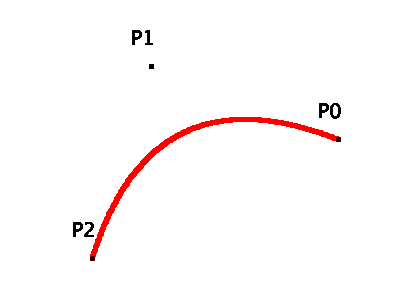
\includegraphics[width=\textwidth]{BC}
		\caption{베지어 곡선}
	\end{subfigure}
	\hfill
	\begin{subfigure}[b]{.45\textwidth}
		\centering
		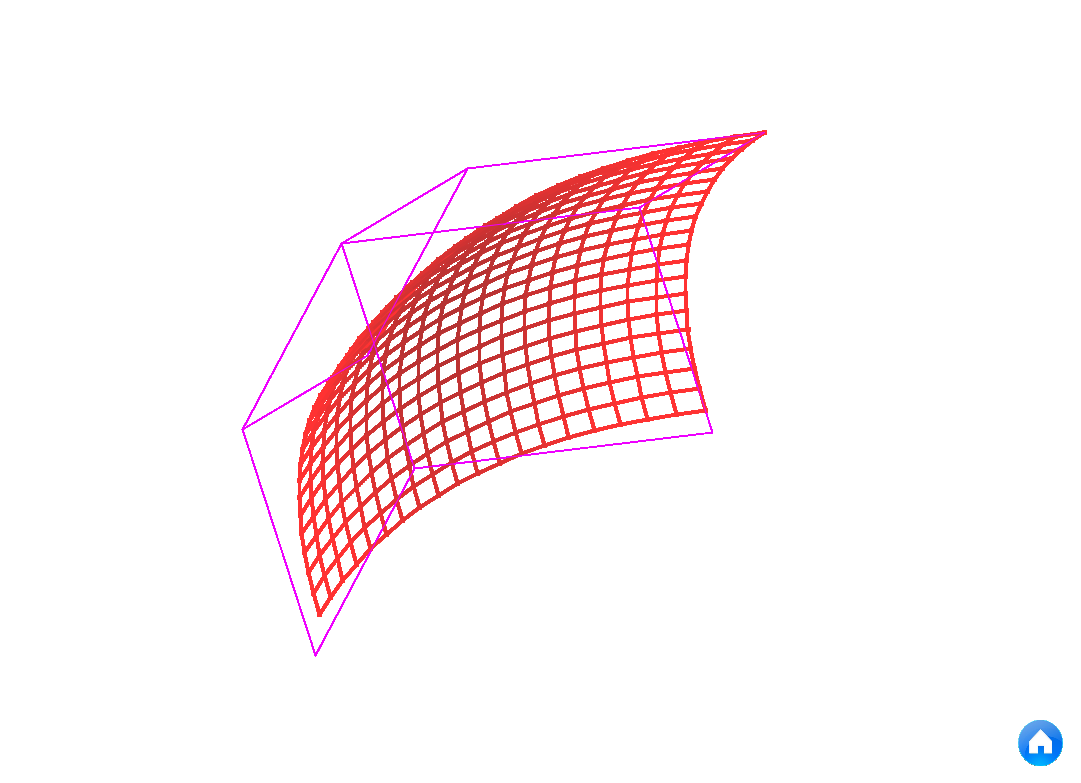
\includegraphics[width=\textwidth]{BS}
		\caption{베지어 곡면}
	\end{subfigure}
	\caption{베지어 곡선(a)과 베지어 곡면(b)}
\end{figure}

\begin{definition} \label{BT}
	벡터 $\mathbf{i}=(i, j, k),\ \mathbf{u}=(u, v, w)$의 표기법을 사용하자. $|\mathbf{i}|=i+j+k=n$이고 Bernstein 다항식은 $B_\mathbf{i}^n(\mathbf{u})=\binom n{i j k}u^iv^jw^k$로 주어진다. 이때 \textbf{$\textbf{n}$차 베지어 삼각형(Bézier triangle)}은 방정식
	\begin{equation}
		\mathbf{x}(\mathbf{u})=\sum_{|\mathbf{i}|=1}B_\mathbf{i}^n(\mathbf{u})\mathbf{b}_\mathbf{i}
	\end{equation}
	에 의한 $\{\mathbf{u}\mid|\mathbf{u}|=1\}$의 상으로 주어진다. 마찬가지로 점 $\mathbf{b}_\mathbf{i}$를 이 베지어 삼각형의 조절점이라 한다.\cite{Farin}
\end{definition}

\begin{figure}[h]
	\centering
	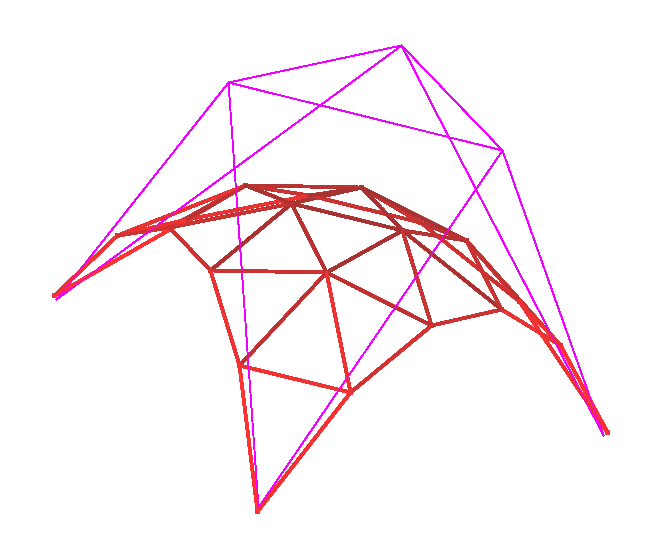
\includegraphics[width=.5\textwidth]{BT}
	\caption{베지어 삼각형}
\end{figure}

베지어 곡면은 특별한 형태의 베지어 곡면이다. 편의상 BT로 표기하자. 

\subsubsection{OBJ와 MTL}
OBJ는 3D 이미지를 저장하는 표준적인 파일이다. OBJ는 3차원 물체를, MTL은 3차원 물체의 색상, 재질, 반사도 등을 저장하는 파일이다. 일반적으로 프로그램을 통해 3차원 모델을 만들면 OBJ와 MTL 파일이 모두 만들어진다. 

우선 OBJ는 정점 $v$, 단위 법선벡터 $v_n$, 텍스쳐 $v_t$, 면 $f$로 이루어진다. 먼저 $v, v_n, v_t$의 $x, y, z$성분이 차례로 주어진다. 마지막에 $f$가 주어지는데, 각각의 $f$는 $v/v_n/v_t$ 블록 3개 또는 4개로 이루어진다. 3개면 삼각형 면, 4개면 사각형 면이다. 아래는 OBJ 파일의 예시이다. 
\begin{Verbatim}
# object heart

v -5.7868 -2.8897 6.9550
v -5.8939 -2.7443 6.7745
...
v 1.3498 1.7948 1.8726
# 5636 vertices

vn -0.3934 -0.8264 -0.4029
...
vn 0.2663 0.7947 -0.5454
# 5634 vertex normals

vt 0.1020 0.1559 0.0000
...
vt 0.7205 0.0233 0.0000
# 5974 texture coordinates

g Heart       # o [object name] / g [group name] 
usemtl Heart  # usemtl [material name]
s 1           # s : smooth
f 1/1/1 2/2991/2 3/1583/3 4/2994/4
...
f 5598/1580/5598 5595/5955/5595 5634/2990/5634 5633/5974/5633
\end{Verbatim}

MTL은 ambient 반사도 $K_a$, diffuse 반사도 $K_d$, specular 반사도 $K_s$ 등으로 이루어진다. 모두 0에서 1 사이의 값을 가지며 각각 물체가 원래 가지고 있는 색에 의한 반사도, 국소적인 색에 의한 반사도, 하이라이트를 일으키는 반사도를 의미한다. 본 연구에서는 $K_a$ 및 $K_d$만 사용했다. 이와 관련해서는 램버트 조명 모델과 함께 설명할 것이다.

\subsubsection{램버트 조명 모델}
\textbf{램버트 조명 모델(Lambertian illumination model)}은 램버트 코사인 법칙에 의한 확산 조명과 환경광에 의한 라이팅을 더한 모델을 말한다.\cite{lambertian model}
\begin{lambert}
	물체 표면에서 반사하는 빛의 휘도는 빛의 입사 벡터 $\mathbf{L}$과 표면의 법선 벡터 $\mathbf{N}$이 이루는 각의 코사인에 비례한다.
\end{lambert}

여기서 $\mathbf{L}$과 $\mathbf{N}$은 단위벡터이며, 따라서 빛의 강도 $I_L$와 물체의 반사 계수 $K_d$에 대해 반사광의 강도는 다음과 같이 주어진다. 
\begin{equation} \label{diffuse light}
	I_d=K_dI_L\cos\theta=K_dI_L(\mathbf{L}\cdot\mathbf{N})
\end{equation}

단 $\cos\theta<0$이라면 법선과 광원이 서로 반대 방향을 향하고 있는 경우이므로 0으로 처리한다. 램버트 코사인 법칙에 따라 얻어진 빛을 \textbf{확산반사광}이라 한다. 이 확산반사광은 음영을 표현하는데 적합하며, 특히 종이처럼 거친 표면에 유용하다.\cite{lambert}\\

\textbf{간접광}은 물체와 여러 차례 반사하며 눈에 들어오는 빛을 의미한다. 그런데 간접광은 정확히 표현하기 어렵다는 문제가 있고, 그래서 만들어진 방식 중 하나가 환경광이다. \textbf{환경광}은 일정한 밝기로 물체를 비추는 빛을 말하며, 물체의 면이나 빛의 방향에 영향을 주지 않는다. 환경광에 의한 식은 다음과 같다.
\begin{equation} \label{ambient light}
	I_a=K_aI_L
\end{equation}

이때 $I_L$는 빛의 강도, $K_a$는 물체의 반사 계수이다. \\

최종적으로 우리 눈에 보이는 색은 환경색와 확산색의 합으로 주어진다.
\begin{enumerate}
\item \textbf{환경색(Ambient color)} $C_a$에 대한 식은 다음과 같다.
\begin{equation} \label{ambient color}
	C_a=C_{material}*I_a
\end{equation}

이 식에서 $I_a$는 \cref{ambient light}에 의해 결정되며 $C_{material}$은 MTL파일에서 주어지는 물체의 색\footnotesize(주어지지 않는 경우 임의로 정의할 수 있다)\normalsize 이다. 이때 각각은 RGB에 대한 벡터로 주어지고 $*$은 각 성분에 대한 곱셈이다. 즉 $(R_1, G_1, B_1)*(R_2, G_2, B_2)=(R_1R_2, G_1G_2, B_1B_2)$

\item \textbf{확산색(Diffuse color)} $C_d$에 대한 식은 다음과 같다.
\begin{equation*} 
	I_d=\frac{K_dI_L(\mathbf{L}\cdot\mathbf{N})}{1+h^2}
\end{equation*}
\begin{equation} \label{diffuse color}
	C_d=C_{material}*I_d
\end{equation}

여기서 $h$는 물체 위의 한 점과 광원 사이의 거리이다. $I_d$는 \cref{diffuse light}에 $1/(1+h^2)$가 추가로 곱해진 형태인데, 이는 점광원을 상정한 결과이다. 기존의 식은 일정한 세기로 평행하게 입사하는 빛의 경우이다. 
\end{enumerate}

우리가 보는 물체의 색 $C$는 다음이 주어진다. 
\begin{equation*}
	C=C_a+C_d=C_{material}*(I_a+I_d)
\end{equation*}

\begin{figure}[h]
	\centering
	\begin{subfigure}{.45\textwidth}
		\centering
		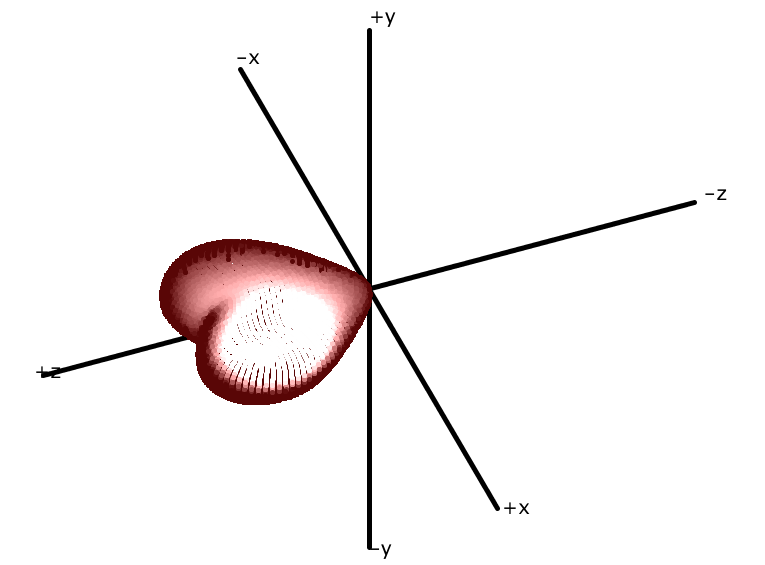
\includegraphics[width=\textwidth]{lambert1}
		\caption{example 1}
	\end{subfigure}
	\hfill
	\begin{subfigure}{.45\textwidth}
		\centering
		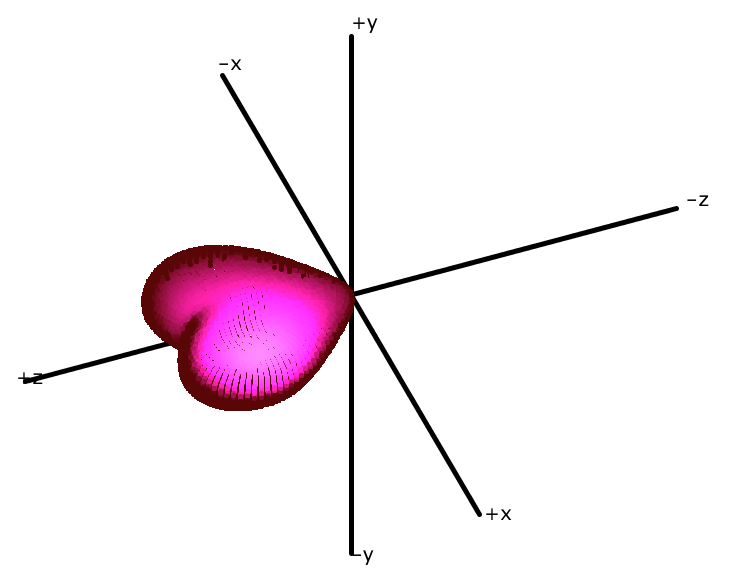
\includegraphics[width=\textwidth]{lambert2}
		\caption{example 2}
	\end{subfigure}
	\caption{램버트 조명 모델의 예시}
\end{figure}

\section{연구 과정}

\subsection{연구 질문}
연구 질문은 다음과 같다:
\begin{enumerate}
	\item 임의의 곡면을 베지어 곡면을 이용해 충분히 근사할 수 있다. (i.e. 오차함수가 0으로 수렴한다)
	\item 곡면 위의 점들이 주어졌을 때 베지어 곡면을 이용해 점들을 충분히 근사할 수 있다. (i.e. 오차함수가 0으로 수렴한다)
	\item OBJ 등 기존의 곡면을 저장하는 방식보다 더 높은 압축 효율을 가진다.
	\item 기존 MTL과 같이 곡면이 지닌 색, 질감 등의 성질도 베지어 곡면의 특징을 이용해 압축하여 저장할 수 있다.
	\item 램버트 조명 모델을 적용하고 베지어 곡면의 움직임을 넣어 조작이 쉽고 입체적인 곡면의 구현을 가능하게 한다.
	\item 근사하거나 구현하는 과정에서 시간이 OBJ보다 적게 소모된다.
	\item 적절한 오차함수를 정의해 근사 정도를 확인하고 기존의 방법보다 오차가 적음을 보인다. 
\end{enumerate}

\subsection{근사 방법}
컴퓨터 그래픽에 사용되는 곡면은 일반적으로 명확한 함수식이 주어지지 않는다. 또 VR 이미지를 저장할 때 곡면 위의 점들의 좌표를 저장하는 경우가 많다. 그래서 실제 VR에 적용될 수 있으려면 곡면 위에 점들이 주어진 상황을 생각해야 한다. 하지만 바로 점들을 근사하는 건 어렵기 때문에 먼저 곡면을 근사하는 방법을 구상하고 점들을 근사하는 방법은 그 다음에 고려할 것이다. 

우리가 사용할 수 있는 건 BS와 BT이다. 구현 시간을 고려해 BS는 $(2,2)$-차, BT는 2차만 사용할 것이다. 이는 4차 이상의 BC가 거의 사용되지 않는 이유와 같다. $(2,2)$-차 BS와 2차 BT 모두 모서리\footnotesize(BS의 경우에는 $u(1-u)v(1-v)=0$, BT의 경우에는 $uv(u+v-1)=0$)\normalsize 가 2차 BC이다. 작년 연구에서 2차 BC로 3차원 곡선을 근사하는 방법을 만들어 놓았기에 그대로 사용할 수 있다. 만들어진 곡면이 끊어지지 않고 연속적으로 이어지기 위해서 모서리 BC는 곡면이 공유하도록 설계할 것이다. 이때 BS는 네 모서리를 결정하는 8개의 조절점이 정해져 우리가 선택할 수 있는 점이 하나가 남고, BT는 세 모서리가 정해지면 모든 점이 결정돼 더 이상 선택할 수 있는 점이 없다. 우리는 BS를 이용한 근사와 BT를 이용한 근사를 모두 시도해볼 예정이다. 컴퓨터 그래픽에서 곡면을 저장할 때 삼각형 분할이 많이 사용되는 만큼 BT에 초점을 맞출 것이다.

\begin{figure}[h]
	\centering
	\begin{subfigure}{.45\textwidth}
		\centering
		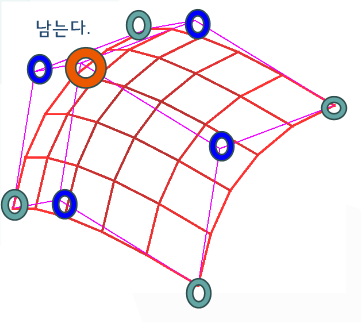
\includegraphics[width=\textwidth]{22BS}
		\caption{$(2,2)$-차 BS}
	\end{subfigure}
	\hfill
	\begin{subfigure}{.45\textwidth}
		\centering
		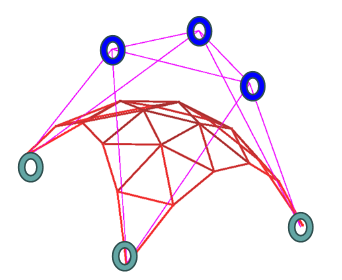
\includegraphics[width=\textwidth]{2BT}
		\caption{2차 BT}
	\end{subfigure}
	\caption{$(2,2)$-차 BS와 2차 BT의 조절점}
	\small $(2,2)$-차 BS(a)는 네 모서리가 결정되면 하나의 조절점만 정할 수 있다. 2차 BT(b)는 세 모서리가 결정되면 모든 조절점이 정해진다. 
\end{figure}

\subsection{OBJ와 비교}
OBJ는 삼/사각형 분할을 통해 곡면을 저장한다.베지어 패치는 삼각형 분할에 비해 매끄러운 표면을 나타내기 적합하고 요구되는 메모리가 적으며 변형을 가하기 쉽다는 장점이 있다. 다만 곡면을 직접 렌더링하기 어렵고, 선과의 교차점을 찾기 어려워 레이트레이싱 등의 기술을 적용하기 어렵다. 

본 연구에서는 베지어 패치의 장점을 살리기 위해 곡면의 모션을 활용할 것이다. 기초 R\&E 연구와 같은 방법을 사용함으로써 구현할 수 있다.\cite{last year, motion}

\subsection{RGB 저장}
이 방법이 실제로 적용되기 위해서는 곡면 자체 뿐만 아니라 색도 저장해야 한다. 색은 RGB로 표현되므로 R, G, B를 각각 저장하는 방식으로 진행할 것이다. 이는 곡면을 이루는 각 점에 어떤 실수 값이 대응된 것으로 생각할 수 있다. 곡면을 $\Phi$라 할 때 $f=r, g, b$에 대해 $f:\Phi\rightarrow\mathbb{R}$라 하자. 이제 우리가 만든 베지어 곡면이 충분히 근사되어 $\Phi$로 간주할 수 있고 베지어 곡면이 매개변수 $u, v$에 대해 $\mathbf{x}(u, v)$로 매개화될 때, $f\circ\mathbf{x}:[0, 1]^2\rightarrow\mathbb{R}$을 생각할 수 있다. 여기서 다음과 같은 두 방법을 떠올렸다.
\begin{enumerate}
	\item 첫번째는 JPG에서 사진을 압축해 저장할 때처럼 색의 변화가 거의 없는 영역을 잡아 색이 일정하다고 놓는 방법이다. 실제로 JPG 파일은 이와 같은 방식으로 RAW 파일을 10배 이상 압축한다. 이 방법은 높은 압축 효율을 기대할 수 있지만 JPG처럼 이미지의 품질이 떨어지거나 노이즈가 발생할 가능성이 크다. 
	
	\item 두번째 방법은 $f\circ\mathbf{x}$의 그래프를 하나의 곡면으로 보고 이를 다시 베지어 곡면으로 압축하는 것이다. 첫번째 방법과 갈리 영역을 잡아 색이 같다고 퉁치지 않기 때문에 정보의 손실이 적고, 조금 더 자연스러운 색감을 얻을 수 있을 것으로 기대된다.
\end{enumerate}

어떤 방식이 더 효과적이고 명확하지 않기 때문에 두 방법을 모두 적용해보고 더 나은 방법을 고를 것이다. 첫번쨰 방법을 구현하기 위해선 JPG 또는 다른 손실 이미지 포맷에 대한 추가적인 공부가 필요하다. 두번째 방법의 경우 색을 저장한다는 특징 때문에 곡면을 저장할 때와는 다른 오차함수가 필요할 수 있다. 

\subsection{오차함수}
작년 연구에서는 오차함수로 하우스도르프 거리를 이용했다.
\begin{definition}
	거리공간 $(M, d)$의 공집합아 아닌 두 부분집합 $X, Y$사이의 하우스도르프 거리는 다음과 같이 주어진다.\cite{Munkres}
	\begin{equation} \label{Hausdorff}
		d_H(X, Y)=\max\left\{\sup_{x\in X}\inf_{y\in Y} d(x, y), \sup_{y\in Y}\inf_{x\in X} d(x, y)\right\}
	\end{equation}
\end{definition}

하우스도르프 거리는 임의의 거리공간에서 두 집합이 서로 떨어진 정도를 나타낸다는 점에서 오차함수로 적절하다.\cite{last year} 그러나 하우스도르프 거리를 곡면에 적용하기에는 문제점이 많다. 기존에는 두 곡선 사이의 하우스도르프 거리를 구하기 위해 구간을 $N$등분해 점들 사이의 거리를 구했는데, 이 경우 시간복잡도가 $O(N^2)$이 된다. 이번에는 곡선이 아니라 곡면이기에 확인해야 하는 변수가 2배 많아지고, 알고리즘의 시간복잡도가 $O(N^4)$으로 제곱이 된다. 그래서 새로운 오차함수를 정의할 필요가 있다. 

\section{연구 결과}
지금까지의 연구 결과를 서술한다.

\subsection{근사 방법}
8진 트리를 이용해 곡면의 근사 방법을 고안했다. \textbf{8진 트리}는 2차원 배열에서의 4진 트리와 비슷하게 3차원 공간상에서 원점을 기준으로 $xy$평면, $yz$평면, $zx$평면으로 잘라 8개로 나누는 것이다. 

8개 조각 중 곡면을 포함하지 않는 건 무시하고, 나머지 조각에서 곡면을 하나의 BT로 근사한다. 그리고 각각의 조각에서 오차함수를 계산해 주어진 $\varepsilon>0$보다 작으면 멈추고, 크면 다시 8개 조각으로 나눠 작업을 계속한다. 이 방법을 통해 충분히 근사 가능함을 오차함수의 정의와 $\varepsilon$-논법을 통해 증명할 것이다. 

\begin{figure}[h]
	\centering
	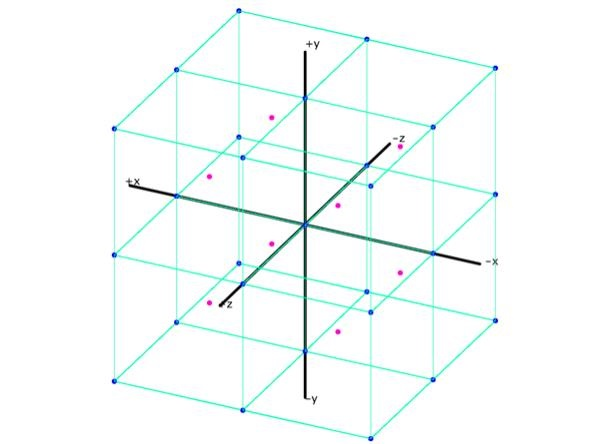
\includegraphics[width=.6\textwidth]{8tree}
	\caption{8진 트리}
	\small 8진트리는 4진트리와 유사하게 3차원 공간을 $xy, yz, zx$평면으로 잘라 8개 노드를 얻는 방식이다. 
\end{figure}

\subsection{오차함수}
우리는 최종적인 연구 목표가 곡면이 아닌 수많은 점들을 근사한다는 것에 착안해 다음과 같은 오차함수를 생각했다. 
\begin{definition} \label{error function}
	공간상의 $N$개의 점 $\mathbf{P}_i\ (i=1, 2, \cdots, N)$을 근사한다고 하자. 점 $\mathbf{P}_i$에서 베지어 곡면까지 $x, y, z$축을 따라 잰 거리를 각각 $\mu_x(\mathbf{P}_i), \mu_y(\mathbf{P}_i), \mu_z(\mathbf{P}_i)$라 할때, 각 점에 대한 오차함수는 다음과 같이 정의한다.
	\begin{equation*}
		\mu(\mathbf{P}_i)=\min\{\mu_x(\mathbf{P}_i), \mu_y(\mathbf{P}_i), \mu_z(\mathbf{P}_i)\}
	\end{equation*}
	
	그리고 오차함수를 다음과 같이 정의한다.
	\begin{equation*}
		\mu=\max\{\mu(\mathbf{P}_i)\mid i=1, 2, \cdots, N\}
	\end{equation*}
\end{definition}

여기서 $\mu_x, \mu_y, \mu_z$를 각각 정의한 이유는 점과 곡면 사이의 최소거리를 직접 구하는 것은 어렵지만 축을 따라 거리를 구하는 것은 쉽기 때문이다. 또 $\mu(\mathbf{P}_i)$를 정의할 때 세 값의 최솟값으로 정의한 이유는 축의 위치에 따라 한 값이 다른 값보다 크게 나올 수 있기 때문이다. 점과 곡면이 쌍곡선 그래프처럼 특이한 위치 관게에 있을 경우 $\mu(\mathbf{P}_i)$값이 실제 곡면까지의 최소 거리보다 크게 얻어질 수 있다. 하지만 그럴 확률은 낮으니 무시할 수 있다.

이후의 연구에서 우리는 \cref{error function}에서 정의한 $\mu$가 오차함수로써 적합한지 알아볼 것이다. 또한 $\mu$ 또는 다른 오차함수에 대해 임의의 점들이 베지어 곡면으로 충분히 근사 가능함을 보일 것이다. 즉 오차함수의 값이 0으로 수렴함을 보일 것이다. 

\section{결론 및 예상 결과}
지금까지의 연구를 통해 램버트 조명 모델을 적용한 애플리케이션(Bézier Modeling Simulator, BMS)을 구현하는데 성공했다. 또 결론에서 제시한 바와 같이 근사 방법의 아이디어를 얻었고 오차함수를 구상했다. 

추가적인 연구를 통해 곡면 위의 점들이 주어진 상태에서 점을 통해 원래 곡면을 근사하는 알고리즘을 완성할 것이다. 또한 서술한 오차함수를 통해 임의의 곡면을 베지어 곡면으로 충분히 근사할 수 있음을 보일 것이다. 즉 근사 알고리즘으로 오차함수가 0에 수렴함을 보인다. 더 나이가 곡면을 근사하여 압축하고, 그 데이터를 통해 빠른 시간 내 곡면을 재구성할 수 있는 애플리케이션 BMS를 만든다. 곡면의 빛 효과, 움직임 등 VR에서 활용도가 높은 기술도 연구하고 적용할 것이다.

지금까지의 과정을 비추어 보았을 때, 다음 학기에 근사 방법을 완성하고 오차함수가 0으로 수렴함을 보일 수 있다. 그리고 OBJ와 달리 베지어 패치를 이용하는 만큼 적지 않은 메모리 감소가 기대된다. 또한 곡면의 움직임을 기초 R\&E연구와 같은 방법으로 진행하면 어렵지 않게 해결할 수 있다. 마지막으로 현재까지 BMS에 많은 부분을 구현해놓았기에 연구를 한층 수월하게 진행할 수 있다. 

이 연구를 통해 VR기술의 큰 발전을 가져올 것으로 기대된다. \\

%%%%%%%%%%%%%%%%%%%%%%%%%%
%%%%%%%%지원 현황%%%%%%%%%
%%%%%%%%%%%%%%%%%%%%%%%%%%

\noindent\fbox{%
    \parbox{\textwidth}{%
    \textbf{
이 보고서는 \researchyearwrite학년도 경기과학고등학교 자율연구의 지원을 받아 제작되었습니다.
}
    }%
}

%%%%%%%%%%%%%%%%%%%%%%%%%%
%%%%%%%%참고 문헌%%%%%%%%%
%%%%%%%%%%%%%%%%%%%%%%%%%%

\begin{thebibliography}{99}
\bibitem{last year} 윤상, 박건호. (2020). \emph{Bezier curve를 이용한 3차원 곡선의 애니메이션화} (기초 R\&E). 경기과학고등학고.
	
\bibitem{Farin} Farin, G. E., \& Farin, G. (2002). \emph{Curves and surfaces for CAGD: a practical guide}. Morgan Kaufmann.

\bibitem{lambertian model} ScienceDirect [Website]. (2021년 6월 21일). URL: \url{https://www.sciencedirect.com/topics/computer-science/lambertian-model}

\bibitem{lambert} Lu, R. (Ed.). (2017). \emph{Light scattering technology for food property, quality and safety assessment}. Crc Press.

\bibitem{motion} 문성룡, 문홍진, 송의남, 김종교. (1985). Quadratic Bezier Polynomial 과 B-Spline Function을 이용한 Curve Fitting 및 Computer Graphic Animation에 관한 기초 연구. \emph{대한전자공학회 학술대회 1985}(1), pp.321-327.

\bibitem{Munkres} Munkres, J. (2014). \emph{Topology}. Pearson Education.

\end{thebibliography}

\end{document}
